\documentclass[pdf]{beamer}
\setbeamertemplate{footline}[frame number]
\setbeamertemplate{section in toc}[sections numbered]
\usepackage{graphicx}
\mode<presentation>{}

\title{The Chinese Head Tax and Chinese Immigration to Canada}
\author{Amy Kim}
\date{September 20, 2022}

\begin{document}
\begin{frame}
    \titlepage
\end{frame}

\begin{frame}{Research Question}
    How did the Chinese Head Tax affect selection into immigration and/or immigrant wealth of Chinese immigrants to Canada in the early 20th century?    
\end{frame}

\begin{frame}{Outline}
    \tableofcontents
\end{frame}

\AtBeginSection[ ]
{
\begin{frame}{Outline}
    \tableofcontents[currentsection]
\end{frame}
}

% BACKGROUND
\section{Background}
\begin{frame}{Background}
    \begin{itemize}
        \item Early 1880s: Influx of Chinese immigrants for construction of Canadian Pacific Railway
        \item 1885: Chinese Exclusion Act institutes \$50 tax
        \begin{itemize}
            \item Only exceptions for students and merchants
            \item Estimated at the time that average annual earnings for 'Chinese laborer' were \$300
        \end{itemize}
        \item Tax raised to \$100 in 1900, \$500 in 1903
        \item In place until 1924, when immigration was banned altogether
        \item Chan (2014) estimates that the Canadian government generated \$23 million in revenue from the Head Tax (approx. 440 million USD today)
    \end{itemize}
\end{frame}

% DATA
\section{Data}
\begin{frame}{Canadian Census Data}
    \centering
    \begin{tabular}{|r||c|c|}
        \hline 
        Year & Coverage & Sampling Method \\
        \hline 
        1852 & 20\% & Random, clustered sample \\
        1871 & 1.8\% & Stratified sample (8 strata)\\
        1881 & 100\% & Full sample \\
        1891 & 5\% & Random sample\footnote{Also includes 10\% of cities and 100\% of all large dwellings and some areas of Ontario} \\
        1901 & 5\% & \textit{Not Specified} \\
        1911 & 5\% & Random sample\footnote{Also includes 10\% of large dwellings and 25\% of multi-unit dwellings} \\
        1921 & 4\% & Random sample\footnote{Also includes 10\% of large dwellings and 20\% of multi-unit dwellings} \\
        \hline
    \end{tabular} \\
    Note: China was not listed as a country of origin in the data until the 1881 census.
\end{frame}

% INITIAL DESCRIPTIVES
\section{Initial Descriptives}
\begin{frame}{Summary Statistics}
    \centering
    \resizebox{0.6\textwidth}{!}{
    \begin{tabular}[]{c|ccc}
        \hline
                & All       & Imm       & Chi \\
        \hline 
                &\multicolumn{3}{c}{1881-1921} \\
        \hline 
        MALE    & 0.52      & 0.57      & 0.97 \\
                & (0.50)    & (0.50)    & (0.16) \\
        MARRIED & 0.354     & 0.54      & 0.51 \\
                & (0.48)    & (0.50)    & (0.50) \\
        AGE     & 26.0      & 36.2      & 34.6 \\
                & (19.4)    & (18.6)    & (11.6) \\
        Obs.    & 5,715,448 & 902,890   & 10,283 \\
        \hline 
                & \multicolumn{3}{c}{1891-1921} \\
        \hline 
        CANREAD & 0.87      & 0.92      & 0.70  \\
                & (0.34)    & (0.27)    & (0.46) \\
        Obs.    & 1,437,638 & 288,321   & 5,967 \\
        \hline 
                & \multicolumn{3}{c}{1901-1921 with nonzero earnings} \\
        \hline 
        EARN    & 708       & 784       & 442 \\
                & (1179)    & (1212)    & (296) \\
        Obs.    & 215,725   & 69,438    & 3,018 \\
        \hline
    \end{tabular}
    }
\end{frame}

\begin{frame}{Percentage of Canadian Immigrants from Various Countries Over Time}
    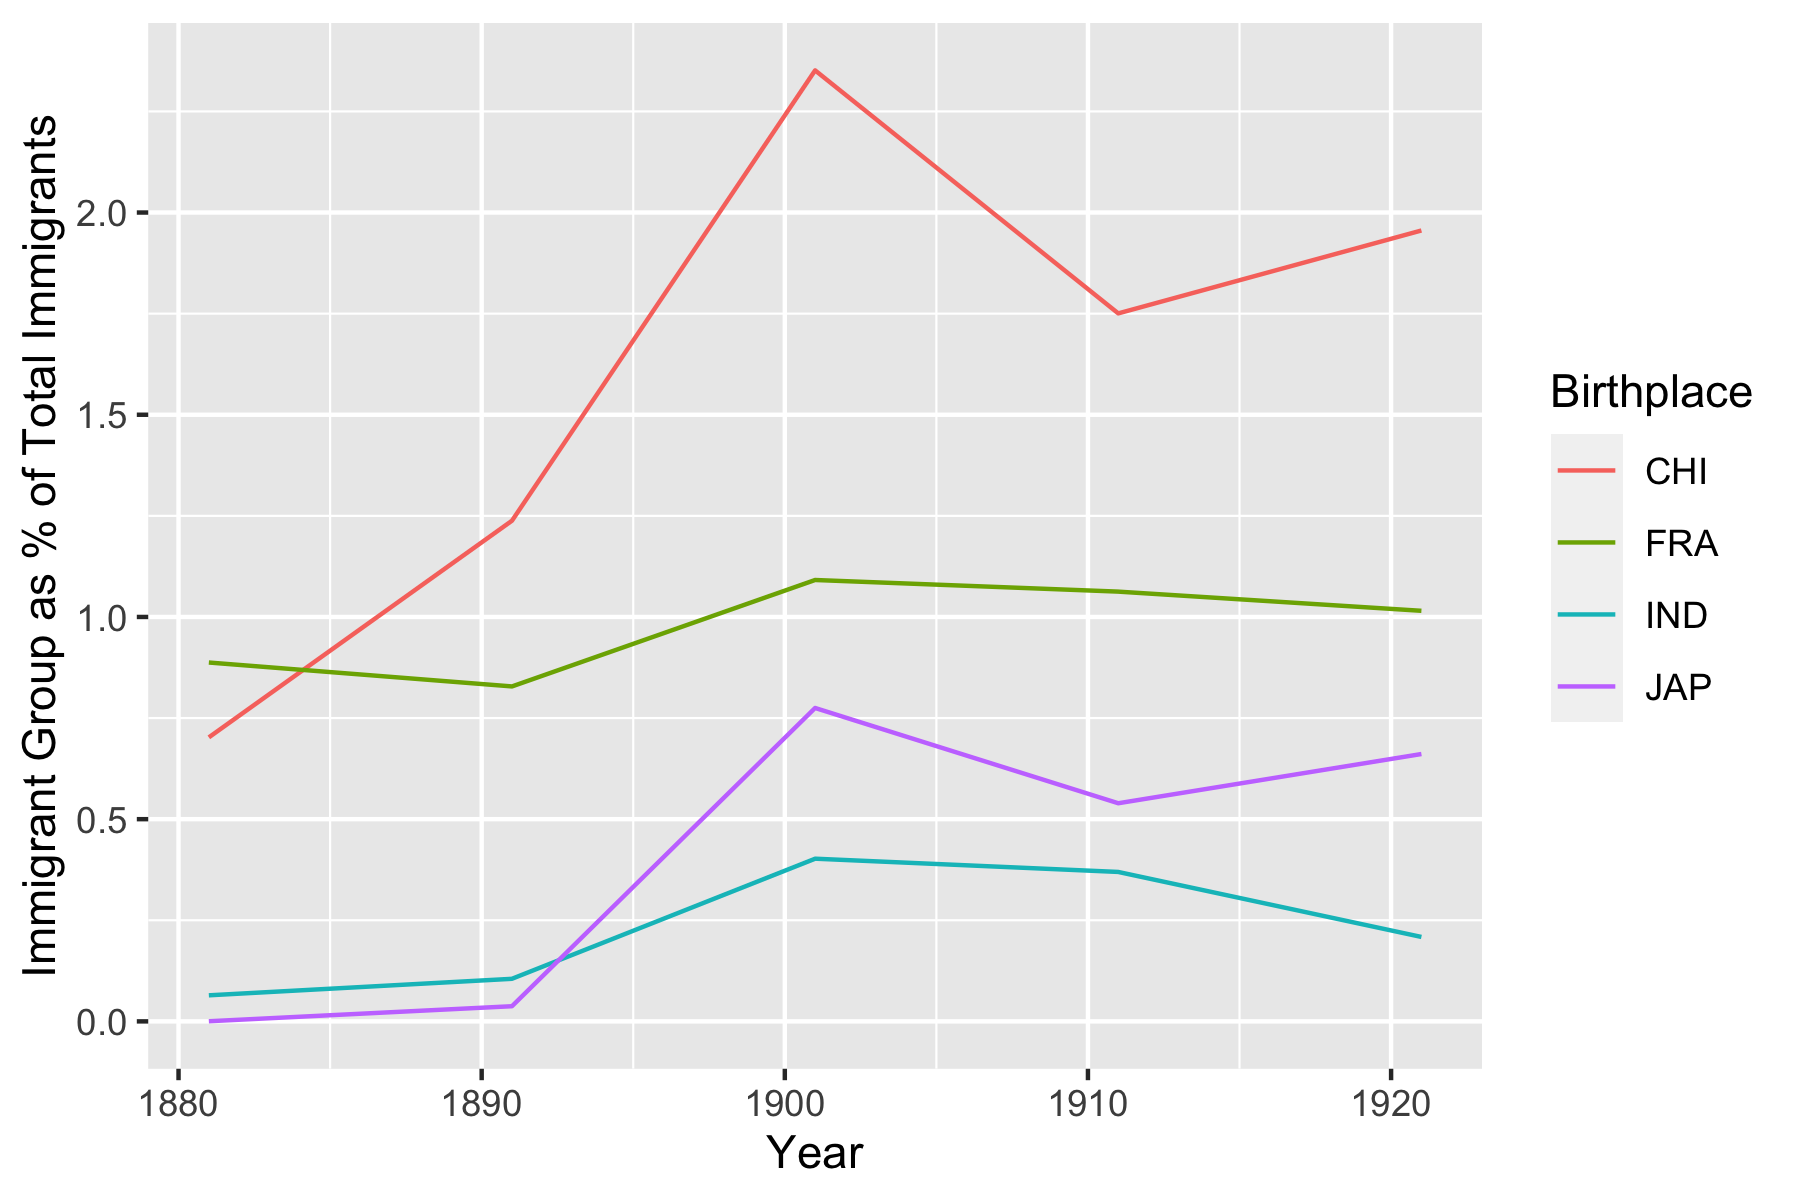
\includegraphics[width = \textwidth]{../../figs/immigpct.png}
\end{frame}

\begin{frame}{Unskilled Workers as a Percentage of All Adult Men for Chinese vs. All Immigrants}
    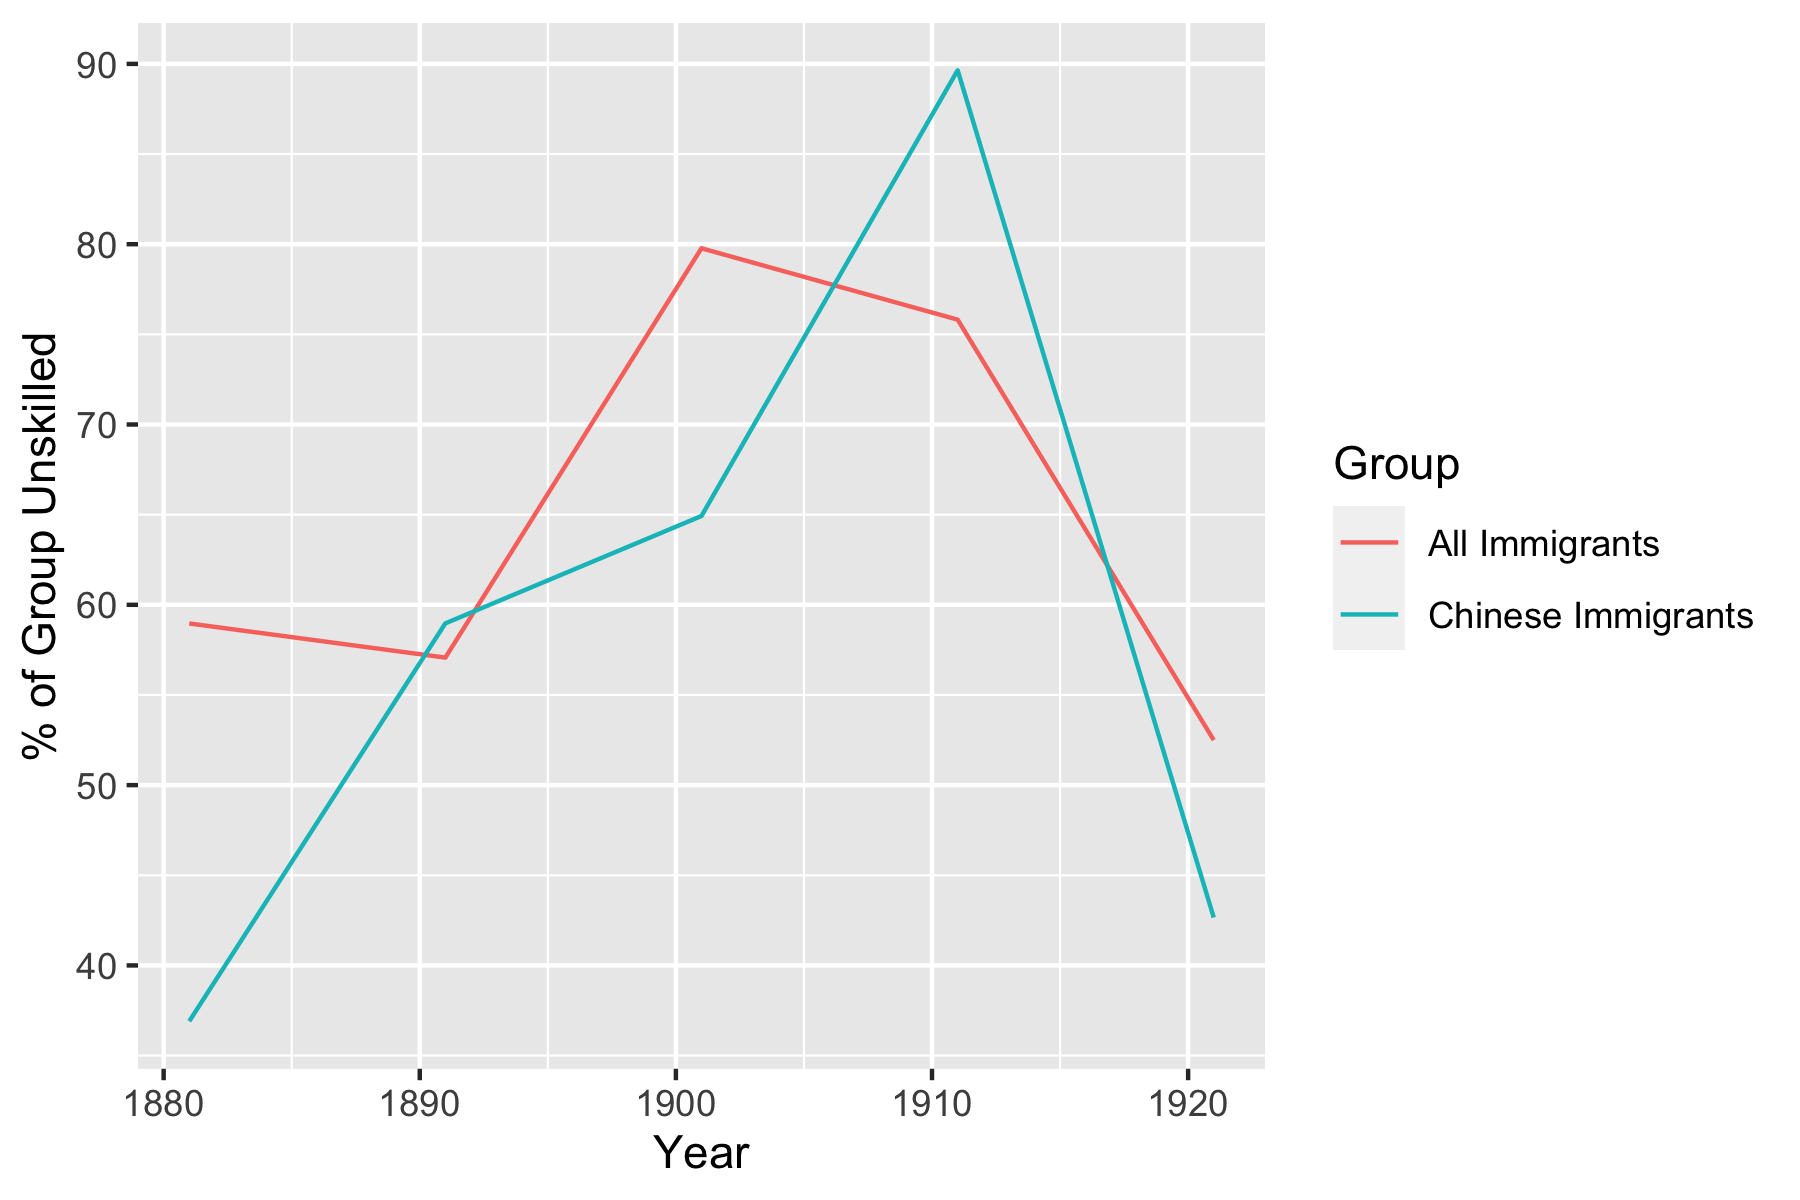
\includegraphics[width = \textwidth]{../../figs/immigocs.png}
\end{frame}

\begin{frame}{Percentage of Canadian Immigrants from China by Year of Immigration for 1901-1921 Censuses}
    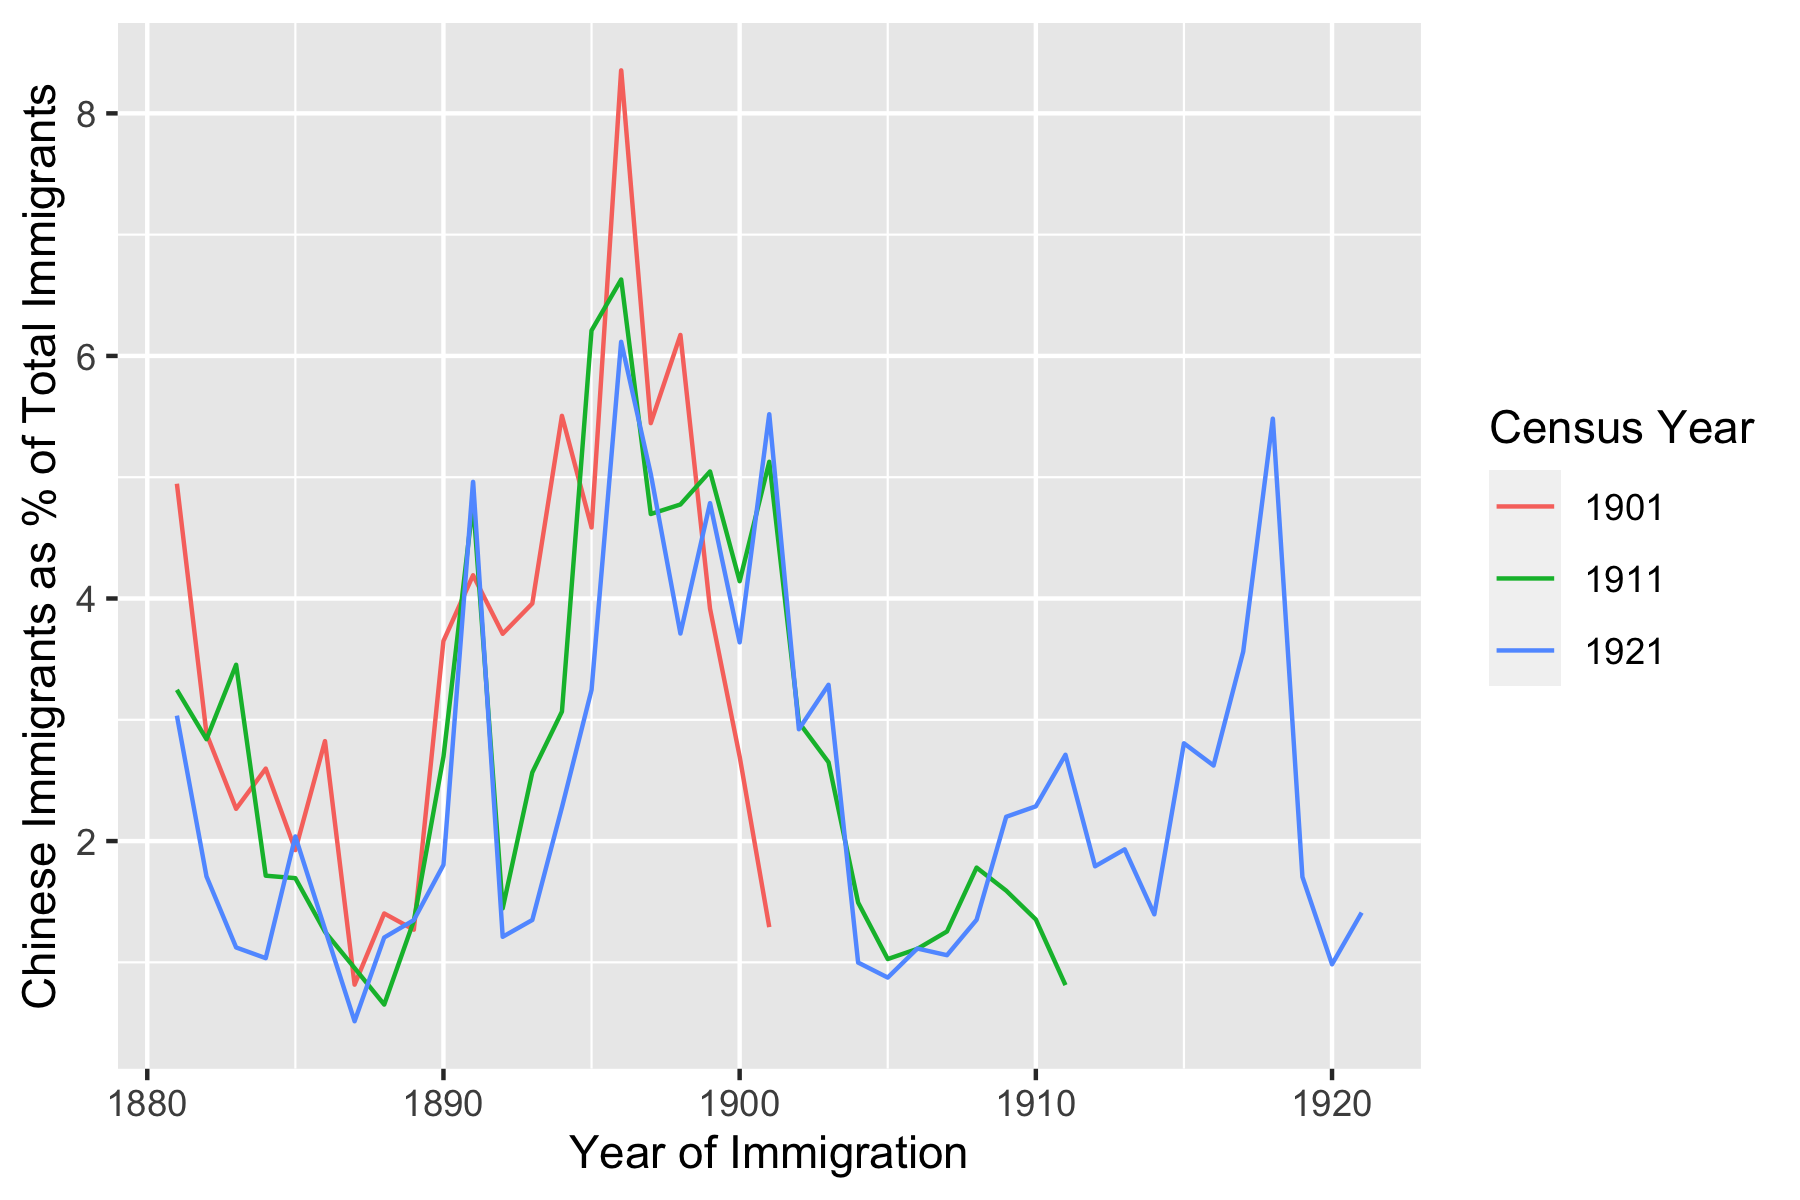
\includegraphics[width = \textwidth]{../../figs/yrimmpct.png}
\end{frame}

\end{document}